\documentclass[a4paper,english]{article}
\usepackage{babel}
\usepackage[utf8]{inputenc}
\usepackage[T1]{fontenc}
\usepackage{times}
\usepackage[pdftex]{graphicx}
\usepackage{color}
\usepackage[pdftex,colorlinks=true,citecolor=black,
            pagecolor=black,linkcolor=black,menucolor=black,
            urlcolor=black]{hyperref}
\usepackage{epstopdf} % addition to include eps
\usepackage{eufrak}
\usepackage{amsmath}
\usepackage{amsbsy}
\usepackage{eucal}
\usepackage{subfigure}
\usepackage{longtable}
\usepackage{url}
\urlstyle{same}
\usepackage{setspace}

\usepackage{natbib}
\usepackage{listings}
\usepackage{algorithm, algorithmic}

\pdfinfo{            
          /Title      (T-61.5110 Modeling of Biological Networks)
          /Author     (Arttu Modig)
          /Keywords   ()          
}


\title{T-61.5110 Modeling of Biological Networks \\ Exercise Session 7}
\author{Arttu Modig \\ 79358S \\
       {\it arttu.modig@aalto.fi}}


\begin{document}
%--- KANSILEHTI -------------------------------------------------------------
\maketitle


%\newpage
%------------------------------------------------------------------------------
\onehalfspacing
\section*{1. Deterministic to Stochastic model conversion}

\begin{figure}
    \begin{center}
        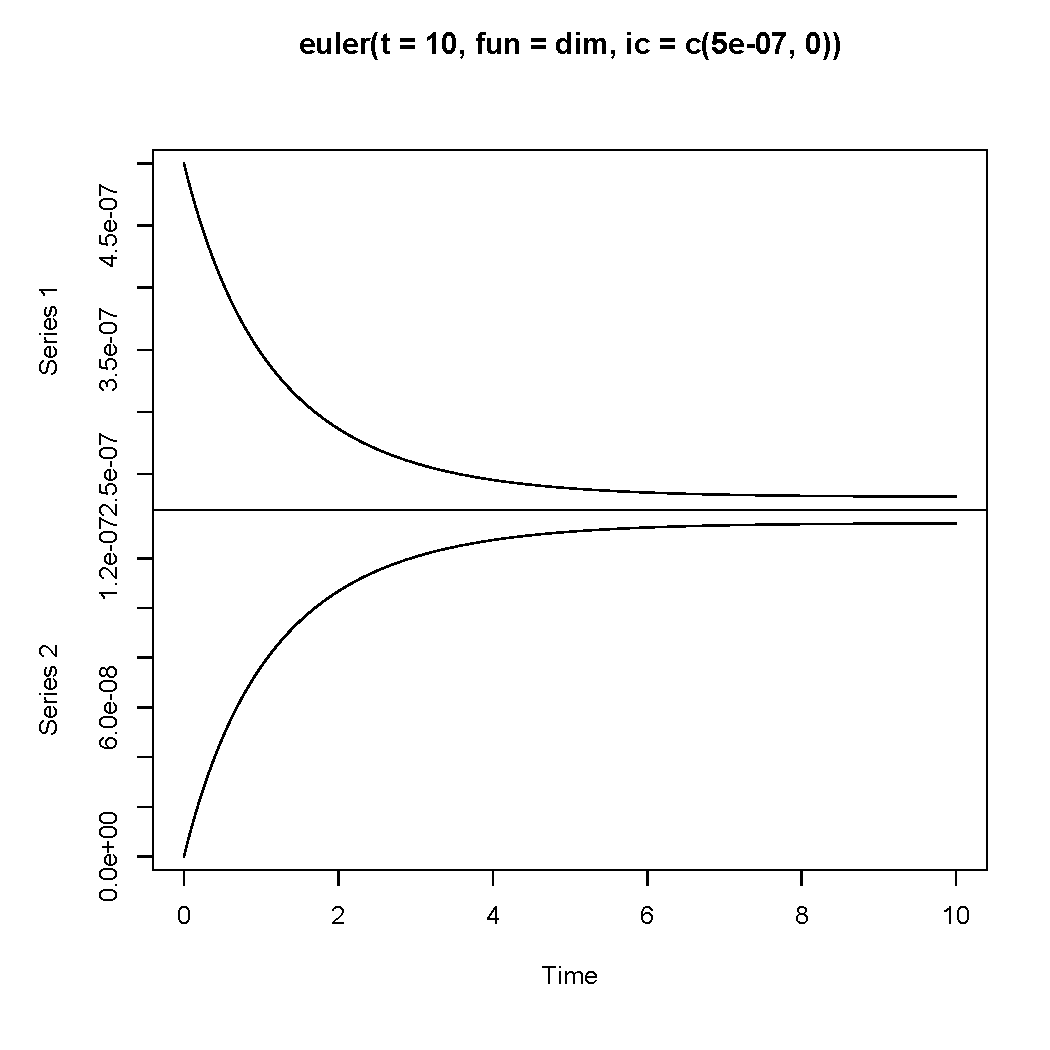
\includegraphics[width=0.5\textwidth]{dimer}
        \caption{The figure shows transitions between two states.}
        \label{rplot}
    \end{center}
\end{figure}

\paragraph{b.}

\begin{figure}
    \begin{center}
        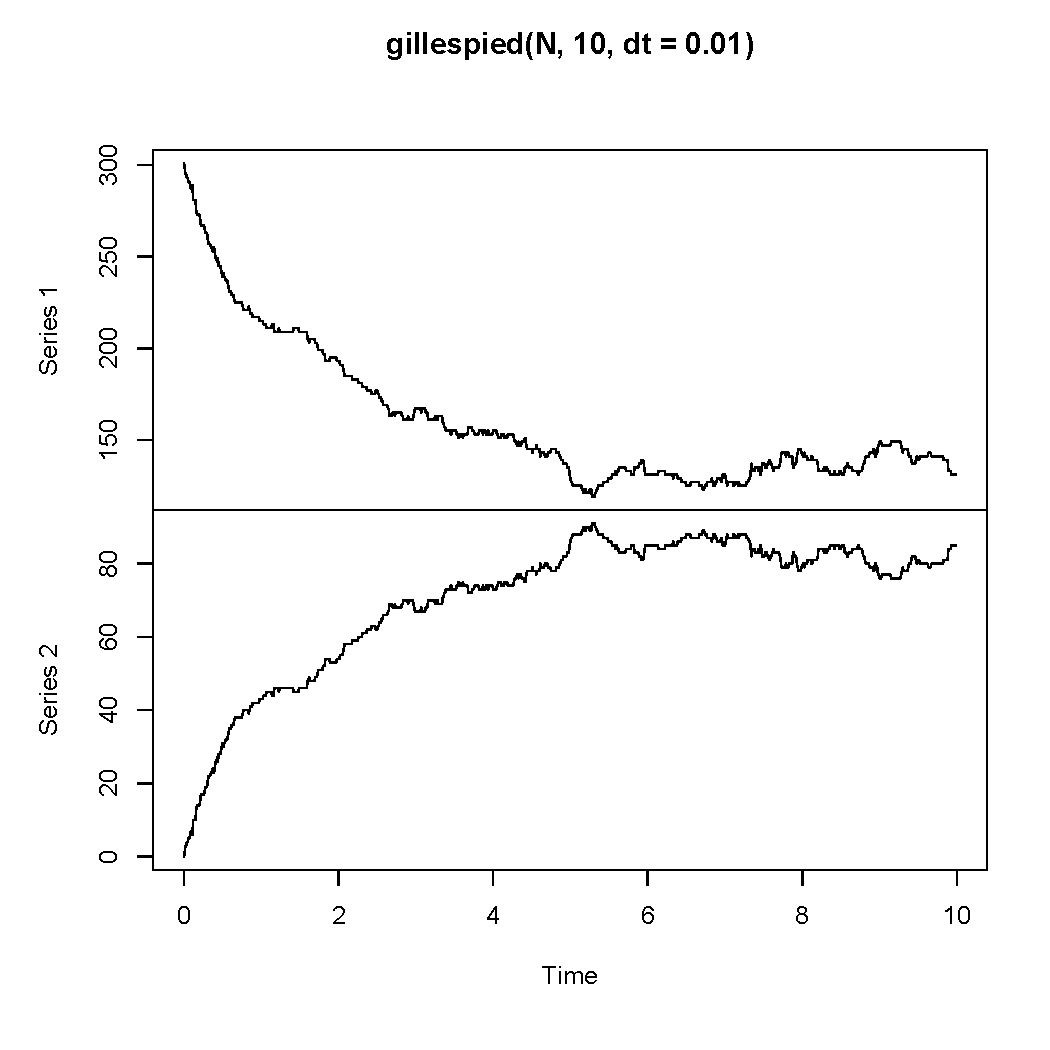
\includegraphics[width=0.5\textwidth]{dimer-stoch}
        \caption{The figure shows transitions between two states.}
        \label{rplot}
    \end{center}
\end{figure}


\paragraph{c.}

\begin{figure}[htp]
  \centering
  \label{figur}\caption{equation...}

  \subfloat[Subcaption 1]{\label{figur:1}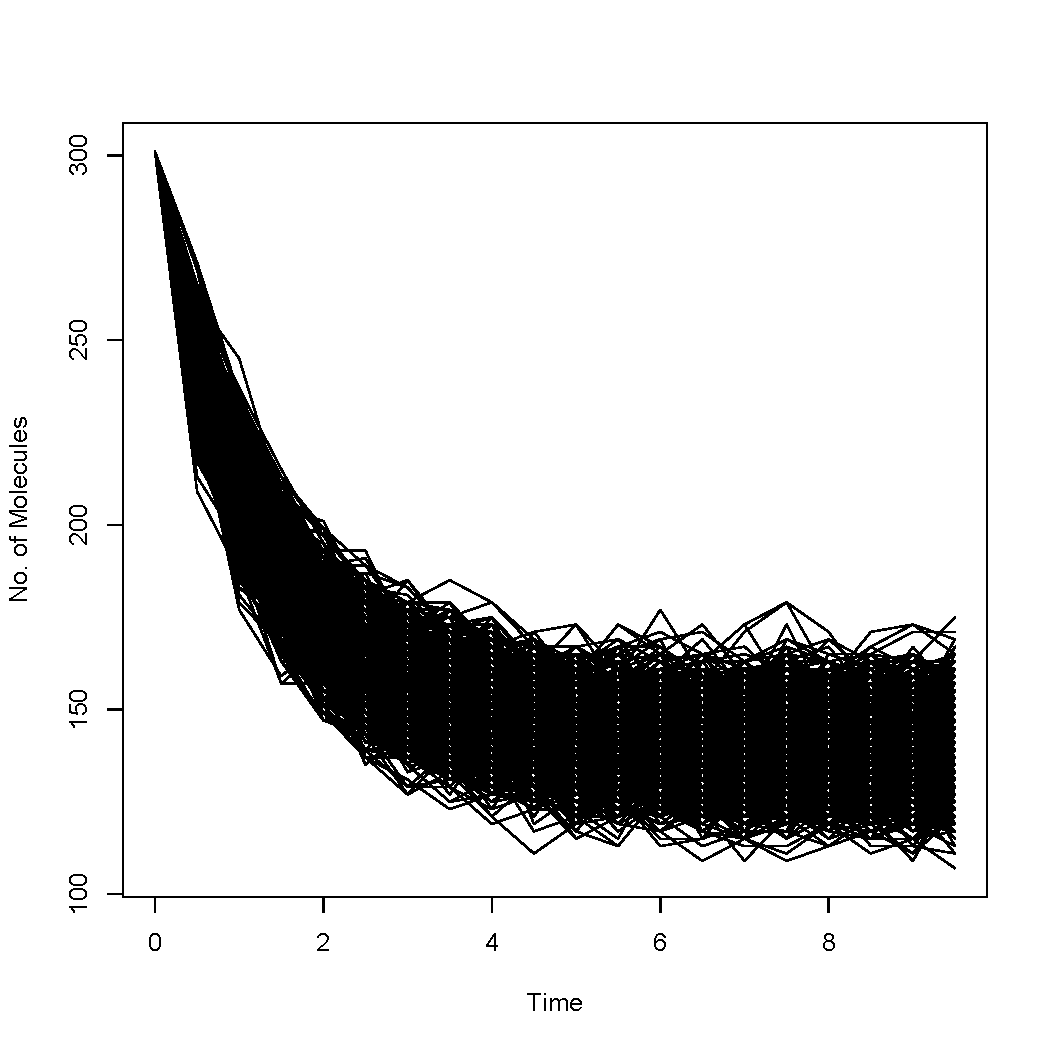
\includegraphics[width=0.3\textwidth]{samples}}
  \subfloat[Subcaption 2]{\label{figur:2}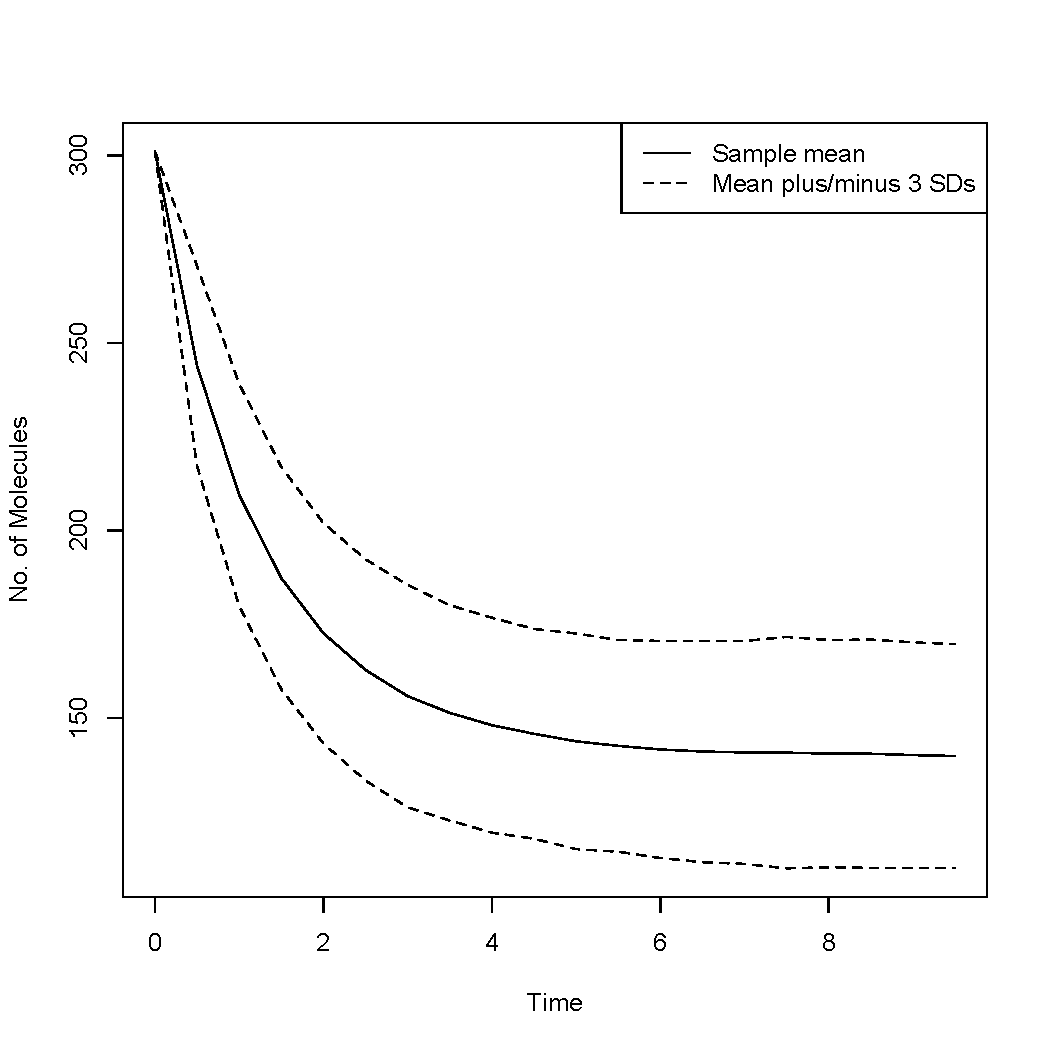
\includegraphics[width=0.3\textwidth]{samplemean}}
  \subfloat[Subcaption 3]{\label{figur:3}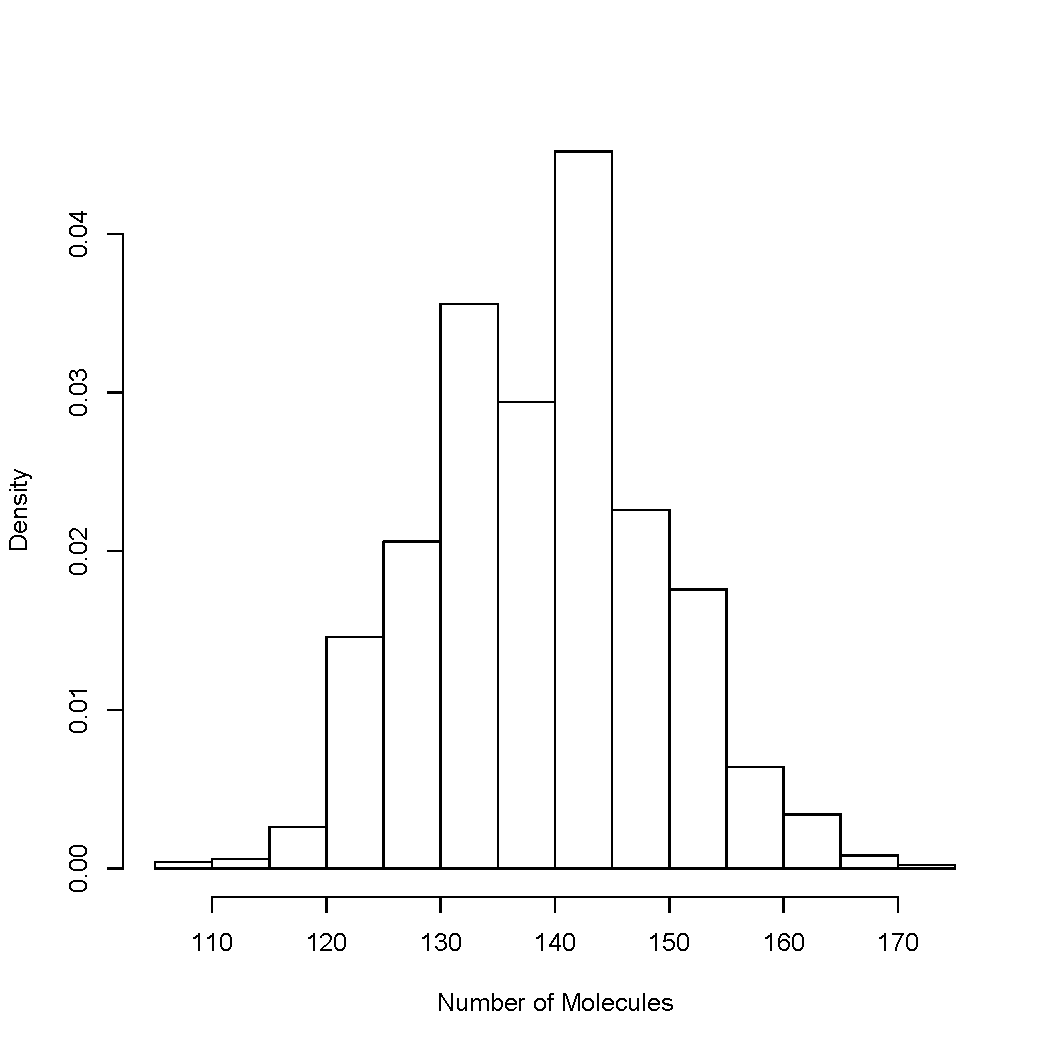
\includegraphics[width=0.3\textwidth]{hist}}

\end{figure}

\section*{2. Stochastic models: Uncertainty and Sensitivity analysis}


\end{document}

%%% Local Variables: 
%%% mode: latex
%%% TeX-master: t
%%% End: 
